\begin{frame}[t]{1D MOC Code}
    
    \begin{itemize}
      \item A transport-based solution that resolves decusping directly with 
      MOC is desired
      \item To aid in developing this method, a 1D MOC code was written
      \begin{itemize}
        \item Able to visualize and analyze angular flux
        \item Simulations with mixed roddded/unrodded cross-sections
        \item Can perform fixed source (fission or total) and eigenvalue 
        calculations
      \end{itemize}
      \item Results provide insights into effects of rod cusping on angular flux
    \end{itemize}
    
\end{frame}

%%%%%%%%%%%%%%%%%%%%%%%%%%%%%%%%%%%%%%%%%%%%%%%%%%%%%%%%%%%%%%%%%%%%%%%%%%%%%%%%%

\begin{frame}[t]{Fixed Total Source}

\begin{columns}
    \begin{column}{0.5\textwidth}
\begin{itemize}
  \item 1D model of VERA Problem 4
  \begin{itemize}
    \item Center row across all 3 assemblies (51 pin cells)
    \item center assembly has 4 partially rodded positions
    \item C5G7 cross-sections \cite{EELewisC5G72003,EELewisC5G7extended2005}
  \end{itemize}
  \item Eigenvalue calculation performed to generate fission and scattering 
  source 
  distributions
  \item MOC sweeps used this source for 0\%, 50\%, and 100\% rodded 
  cross-sections
\end{itemize}
\end{column}
\begin{column}{0.28\textwidth}
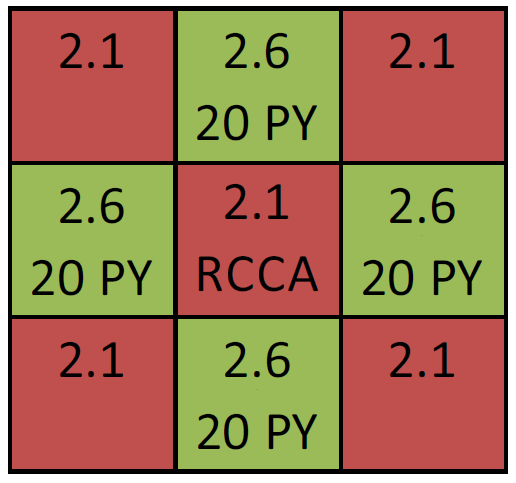
\includegraphics[width=\textwidth]{p4a_layout.png}
\end{column}
\begin{column}{0.22\textwidth}
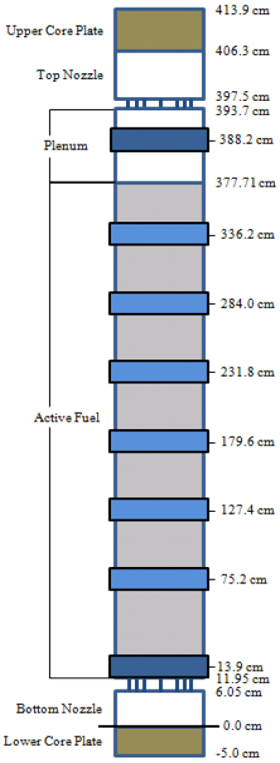
\includegraphics[width=\textwidth]{wb_3d_assembly.png}
\end{column}
\end{columns}

\end{frame}

%%%%%%%%%%%%%%%%%%%%%%%%%%%%%%%%%%%%%%%%%%%%%%%%%%%%%%%%%%%%%%%%%%%%%%%%%%%%%%%%%

\begin{frame}[t]{Fixed Total Source}

\begin{figure}[H]
    \centering
    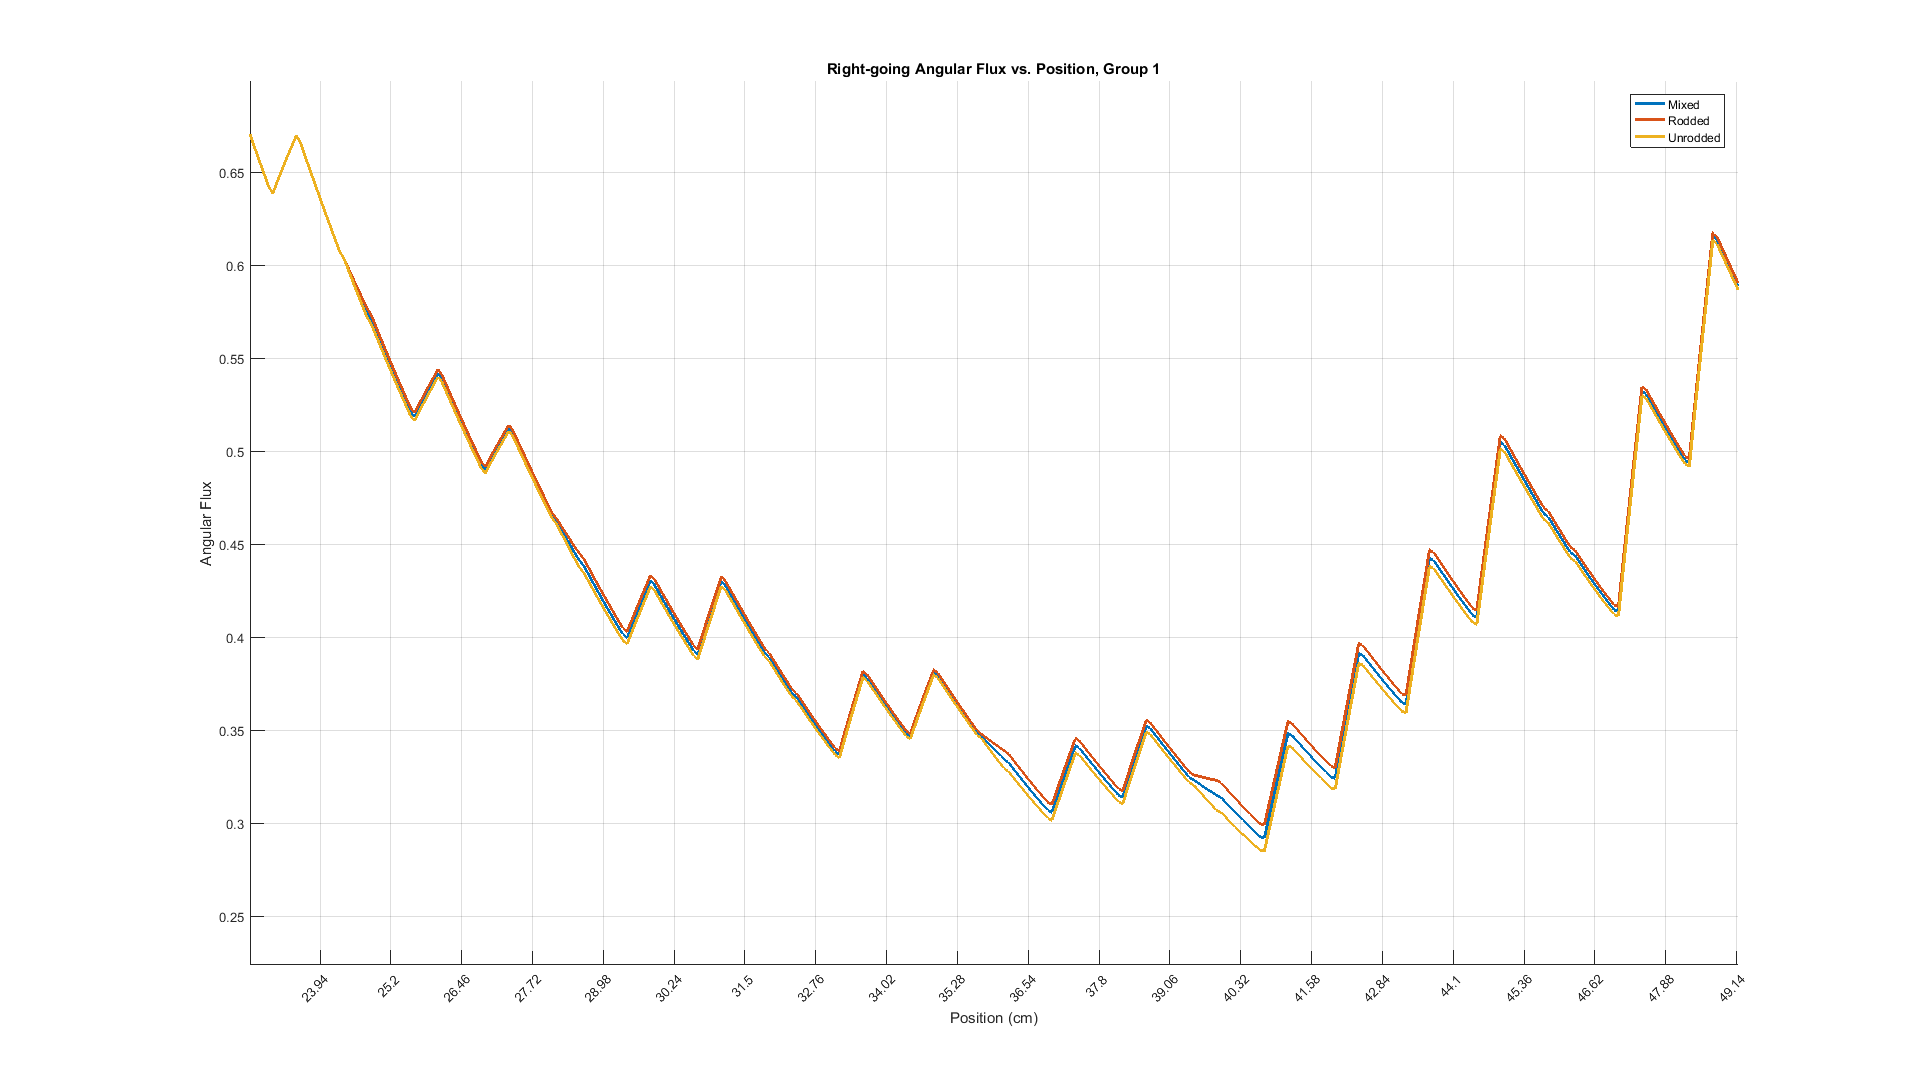
\includegraphics[width=0.6\textwidth]{../figs/1dmoc-50mix-fixedscat-angflux1.png}
\end{figure}
\begin{itemize}
  \item Fast flux differences are small but build up
\end{itemize}

\end{frame}

%%%%%%%%%%%%%%%%%%%%%%%%%%%%%%%%%%%%%%%%%%%%%%%%%%%%%%%%%%%%%%%%%%%%%%%%%%%%%%%%%

\begin{frame}[t]{Fixed Total Source}

\begin{figure}[H]
  \centering
  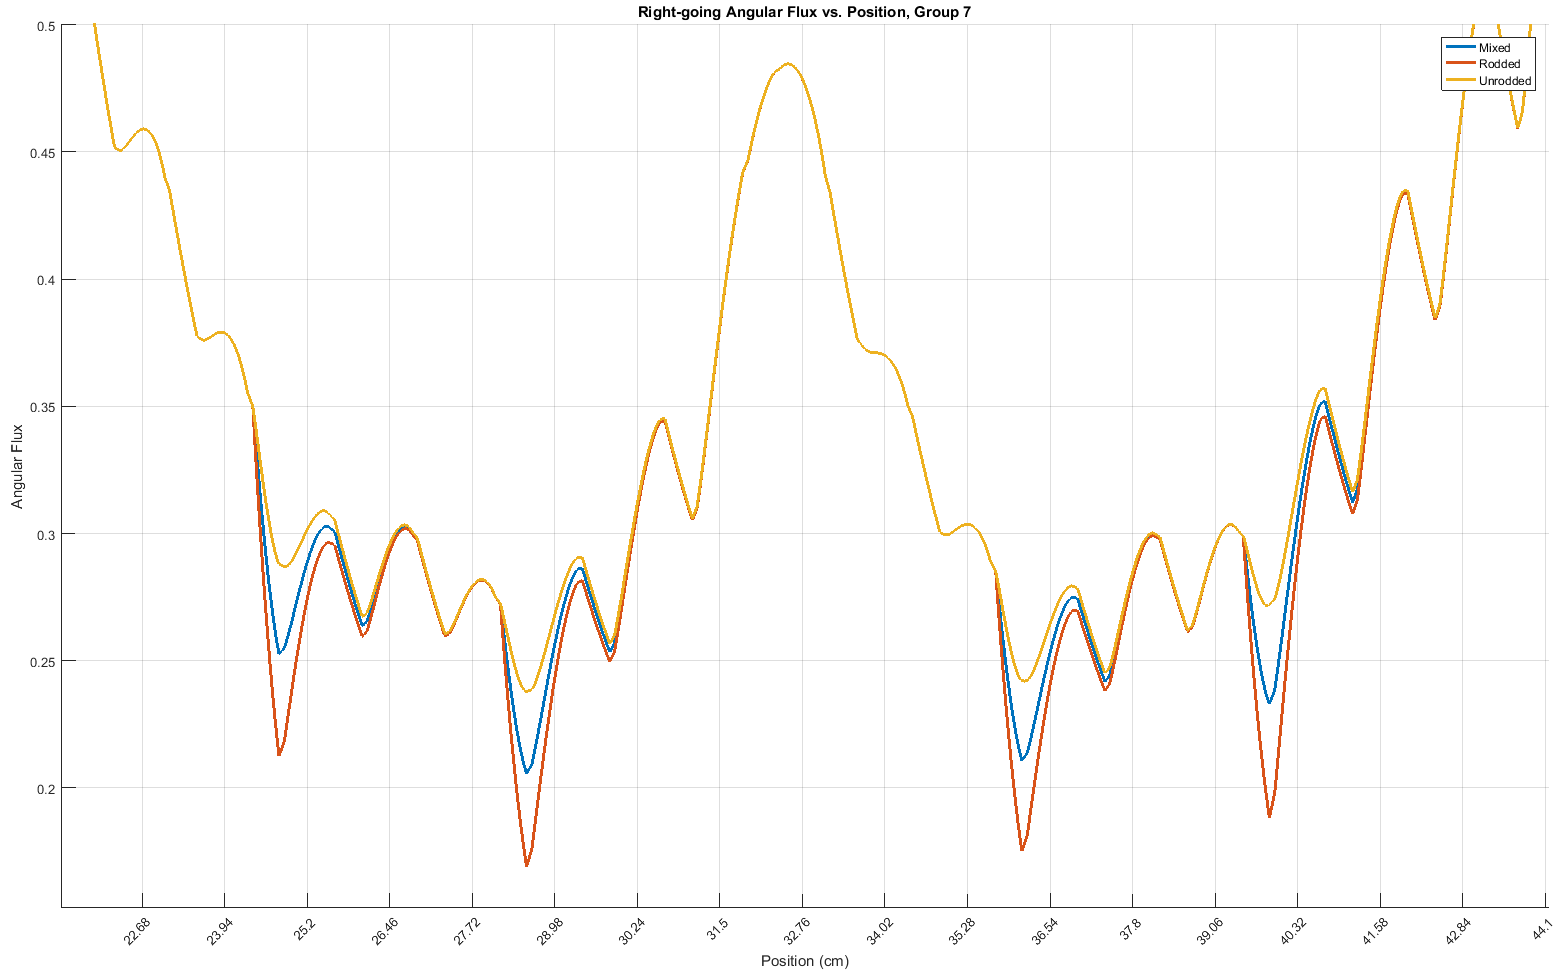
\includegraphics[width=0.6\textwidth]{../figs/1dmoc-50mix-fixedscat-angflux7.png}
\end{figure}
\begin{itemize}
  \item Thermal flux differences are large but dissipate quickly
\end{itemize}

\end{frame}

%%%%%%%%%%%%%%%%%%%%%%%%%%%%%%%%%%%%%%%%%%%%%%%%%%%%%%%%%%%%%%%%%%%%%%%%%%%%%%%%%

\begin{frame}[t]{Fixed Total Source}

\begin{figure}[H]
    \centering
    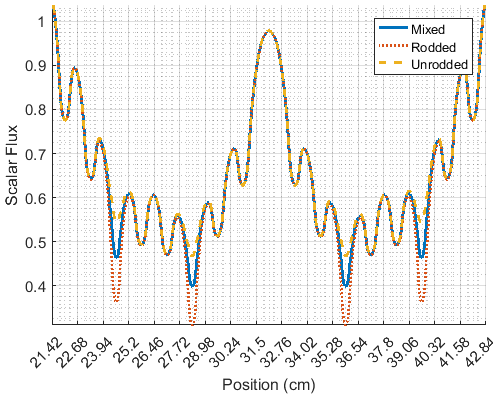
\includegraphics[width=0.7\textwidth]{../figs/1dmoc-50mix-fixedscat-scalflux7.png}
    \caption{Group 7 scalar flux comparisons for a fixed fission and scattering source calculation}\label{f:1dmoc-fixed-50-scalflux7}
\end{figure}

\end{frame}

%%%%%%%%%%%%%%%%%%%%%%%%%%%%%%%%%%%%%%%%%%%%%%%%%%%%%%%%%%%%%%%%%%%%%%%%%%%%%%%%%

\begin{frame}[t]{Fixed Fission Source}
    
    \begin{columns}
        \begin{column}{0.5\textwidth}
    \begin{itemize}
      \item 1D model of VERA Problem 4
      \item Eigenvalue calculation performed to generate fission source
      \item Calculations performed using 25\%, 50\%, and 75\% rodded 
      cross-sections
      \begin{itemize}
        \item Same, fixed fission source for each case
        \item Multiple iterations allowed for each case to converge scattering 
        source
      \end{itemize}
    \end{itemize}
\end{column}
\begin{column}{0.28\textwidth}
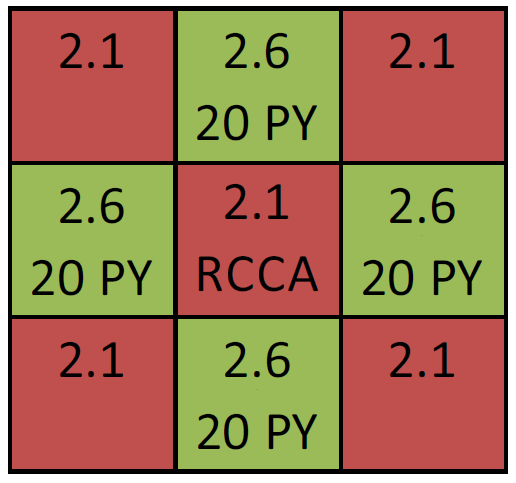
\includegraphics[width=\textwidth]{p4a_layout.png}
\end{column}
\begin{column}{0.22\textwidth}
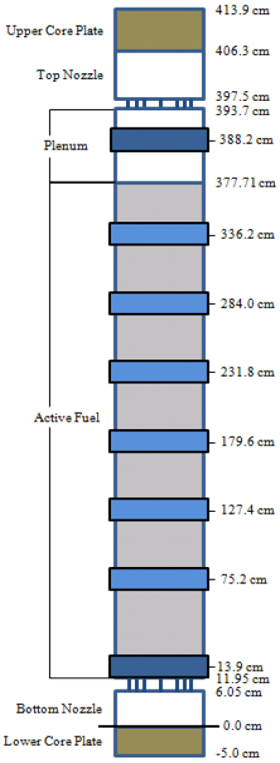
\includegraphics[width=\textwidth]{wb_3d_assembly.png}
\end{column}
\end{columns}
    
\end{frame}

%%%%%%%%%%%%%%%%%%%%%%%%%%%%%%%%%%%%%%%%%%%%%%%%%%%%%%%%%%%%%%%%%%%%%%%%%%%%%%%%%

\begin{frame}[t]{Fixed Fission Source}

\begin{columns}
    \begin{column}{0.6\textwidth}
\begin{itemize}
  \item Angular Flux, Group 7, 25\% rodded
\end{itemize}
\begin{figure}[H]
    \centering
    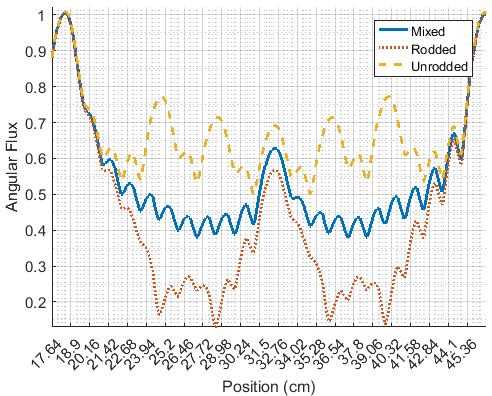
\includegraphics[width=\textwidth]{1dmoc-25mix-angflux7.png}
\end{figure}
\end{column}
\begin{column}{0.4\textwidth}
\begin{figure}[H]
    \centering
    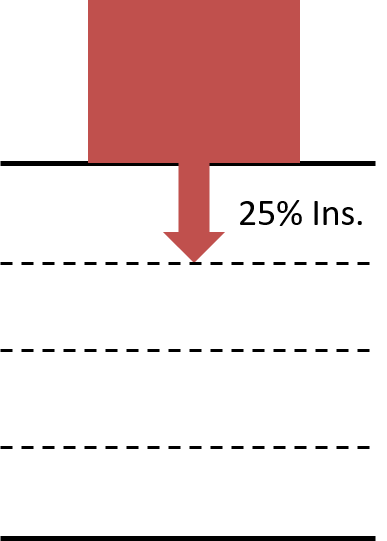
\includegraphics[width=0.75\textwidth]{rodInsertion-25percent.png}
\end{figure}
\end{column}
\end{columns}

\end{frame}

%%%%%%%%%%%%%%%%%%%%%%%%%%%%%%%%%%%%%%%%%%%%%%%%%%%%%%%%%%%%%%%%%%%%%%%%%%%%%%%%%

\begin{frame}[t]{Fixed Fission Source}

\begin{columns}
    \begin{column}{0.6\textwidth}
        \begin{itemize}
            \item Angular Flux, Group 7, 50\% rodded
        \end{itemize}
        \begin{figure}[H]
            \centering
            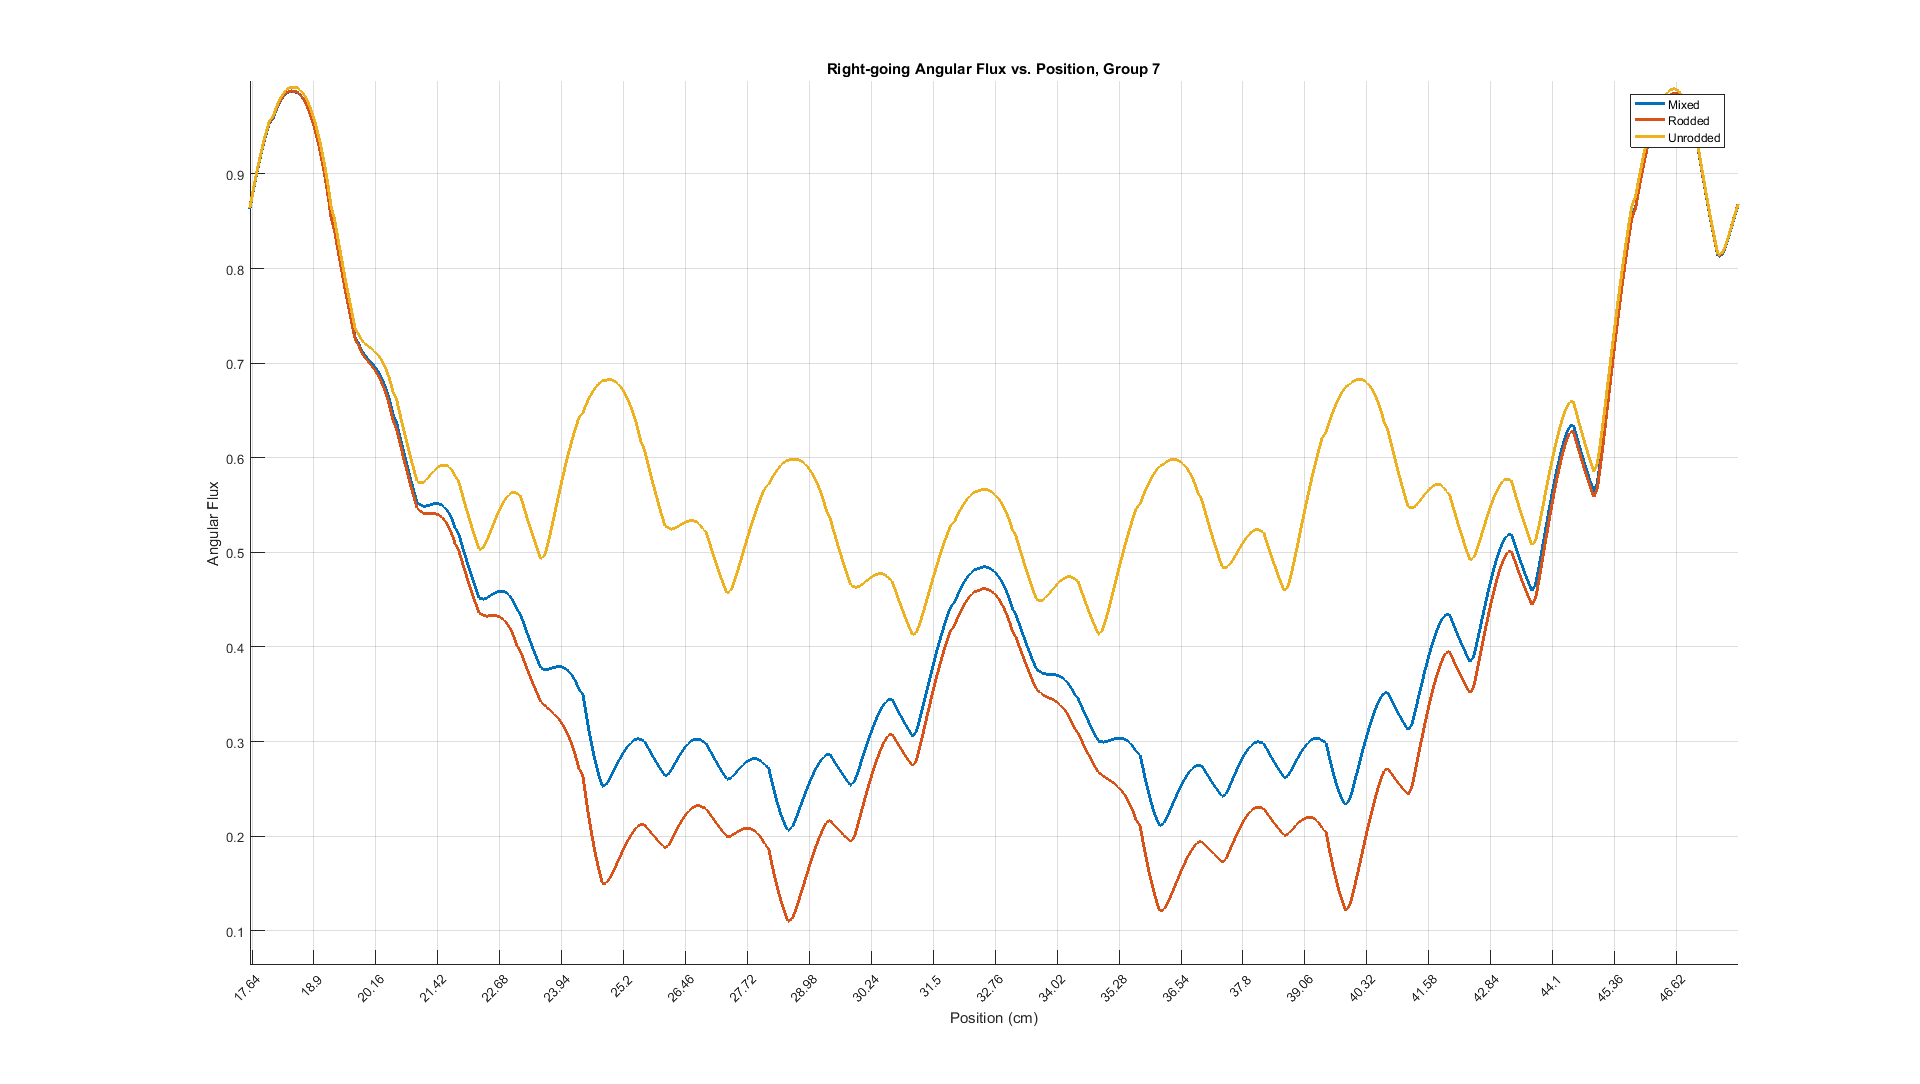
\includegraphics[width=\textwidth]{1dmoc-50mix-angflux7.png}
        \end{figure}
    \end{column}
    \begin{column}{0.4\textwidth}
        \begin{figure}[H]
            \centering
            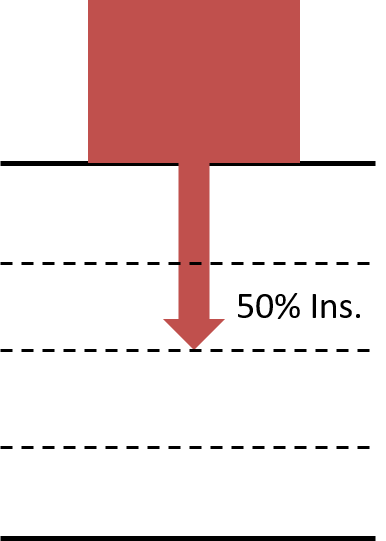
\includegraphics[width=0.75\textwidth]{rodInsertion-50percent.png}
        \end{figure}
    \end{column}
\end{columns}

\end{frame}

%%%%%%%%%%%%%%%%%%%%%%%%%%%%%%%%%%%%%%%%%%%%%%%%%%%%%%%%%%%%%%%%%%%%%%%%%%%%%%%%%

\begin{frame}[t]{Fixed Fission Source}

\begin{columns}
    \begin{column}{0.6\textwidth}
        \begin{itemize}
            \item Angular Flux, Group 7, 75\% rodded
        \end{itemize}
        \begin{figure}[H]
            \centering
            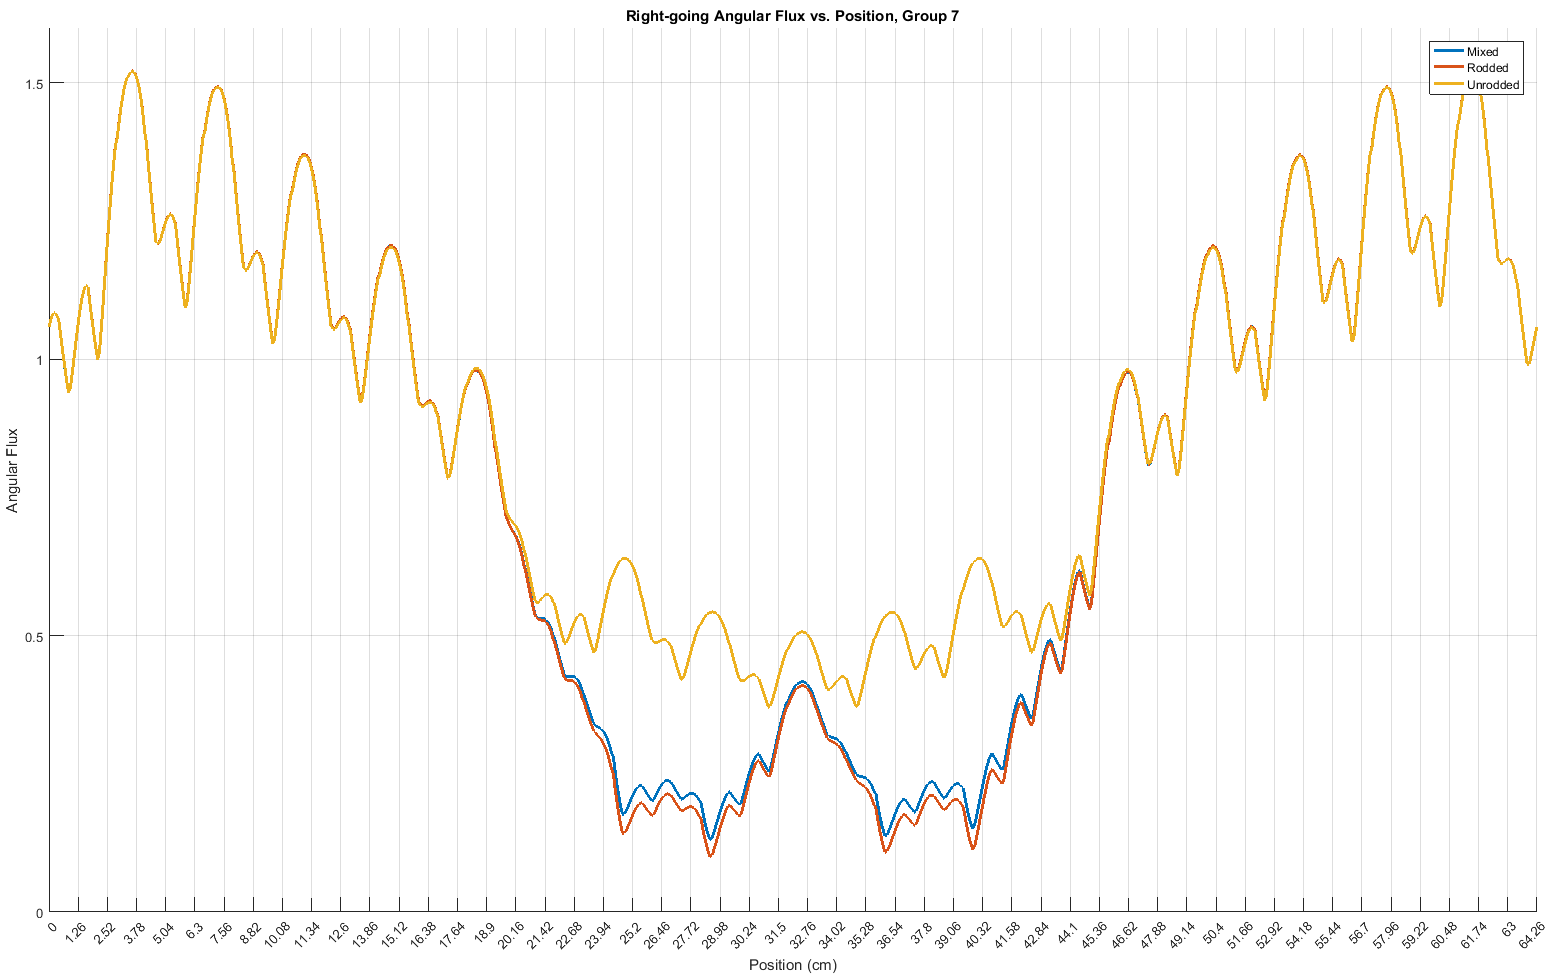
\includegraphics[width=\textwidth]{1dmoc-75mix-angflux7.png}
        \end{figure}
    \end{column}
    \begin{column}{0.4\textwidth}
        \begin{figure}[H]
            \centering
            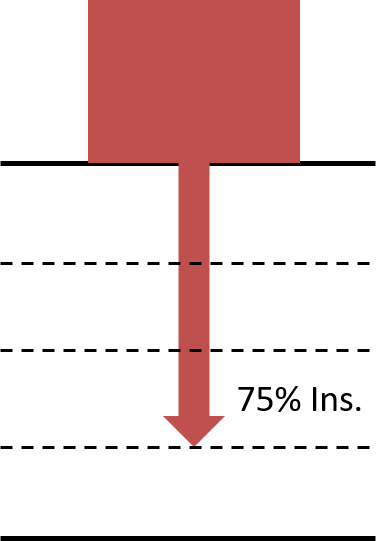
\includegraphics[width=0.75\textwidth]{rodInsertion-75percent.png}
        \end{figure}
    \end{column}
\end{columns}

\end{frame}

%%%%%%%%%%%%%%%%%%%%%%%%%%%%%%%%%%%%%%%%%%%%%%%%%%%%%%%%%%%%%%%%%%%%%%%%%%%%%%%%%

\begin{frame}[t]{Fixed Fission Source}

\begin{columns}
    \begin{column}{0.6\textwidth}
        \begin{itemize}
            \item Angular Flux, Group 1, 25\% rodded
        \end{itemize}
        \begin{figure}[H]
            \centering
            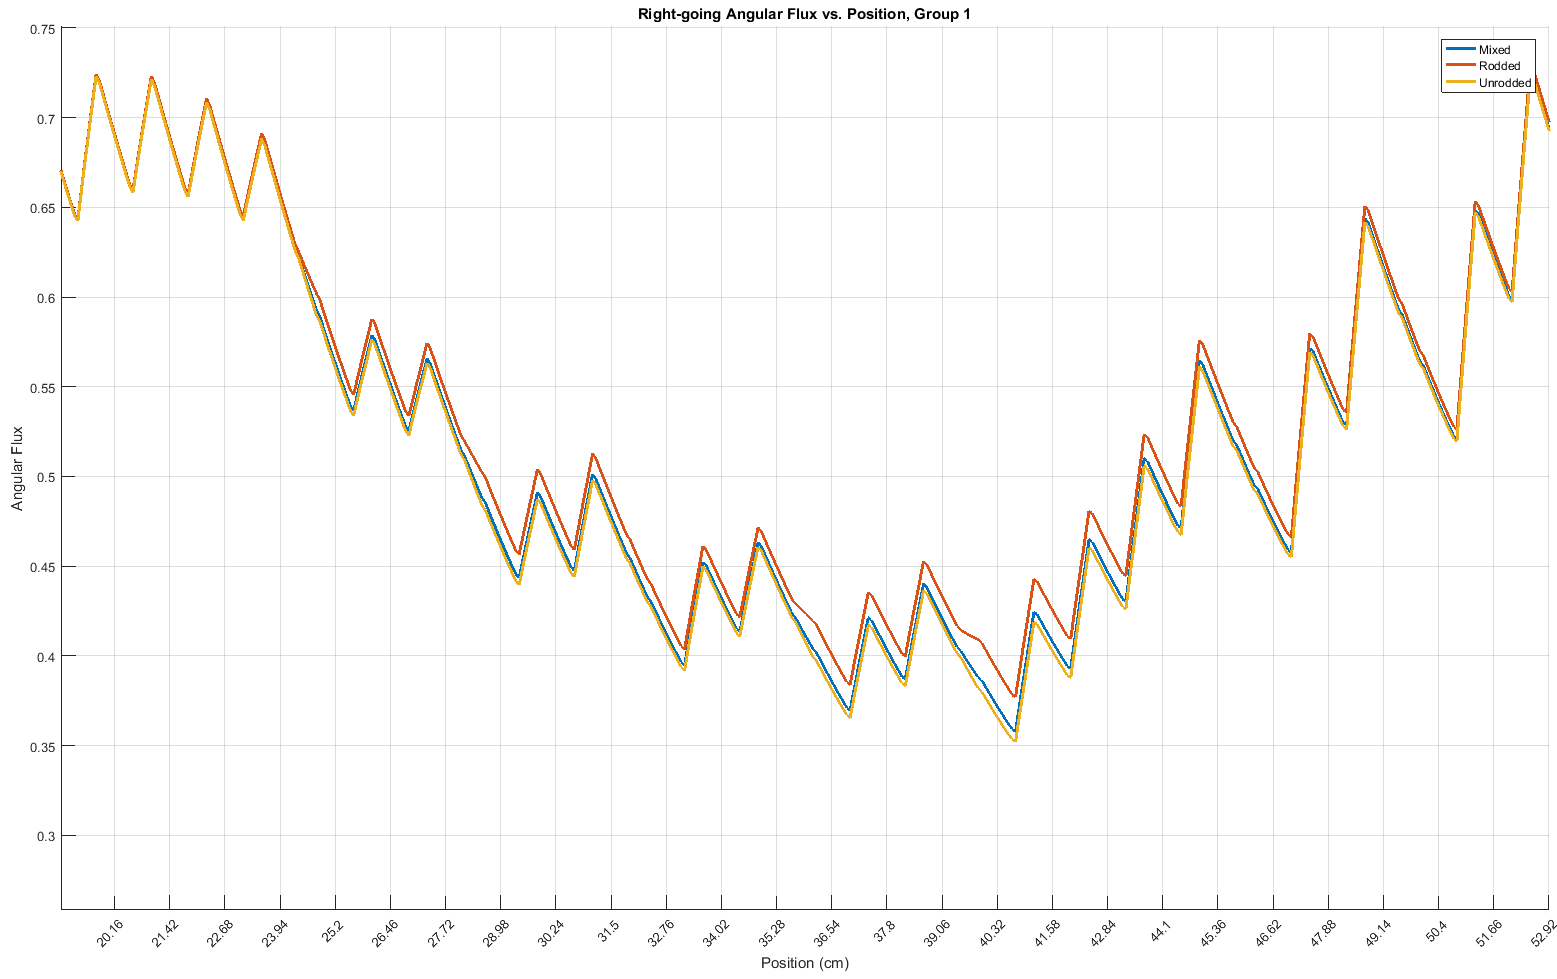
\includegraphics[width=\textwidth]{1dmoc-25mix-angflux1.png}
        \end{figure}
    \end{column}
    \begin{column}{0.4\textwidth}
        \begin{figure}[H]
            \centering
            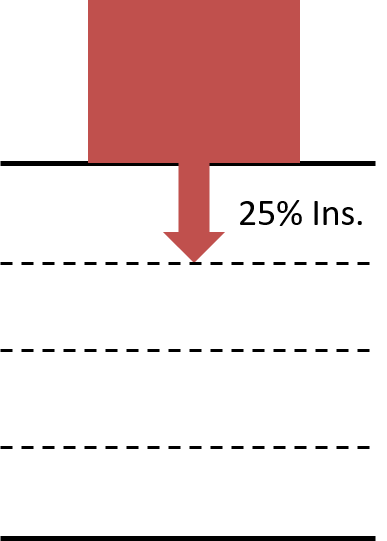
\includegraphics[width=0.75\textwidth]{rodInsertion-25percent.png}
        \end{figure}
    \end{column}
\end{columns}

\end{frame}

%%%%%%%%%%%%%%%%%%%%%%%%%%%%%%%%%%%%%%%%%%%%%%%%%%%%%%%%%%%%%%%%%%%%%%%%%%%%%%%%%

\begin{frame}[t]{Fixed Fission Source}

\begin{columns}
    \begin{column}{0.6\textwidth}
        \begin{itemize}
            \item Angular Flux, Group 1, 50\% rodded
        \end{itemize}
        \begin{figure}[H]
            \centering
            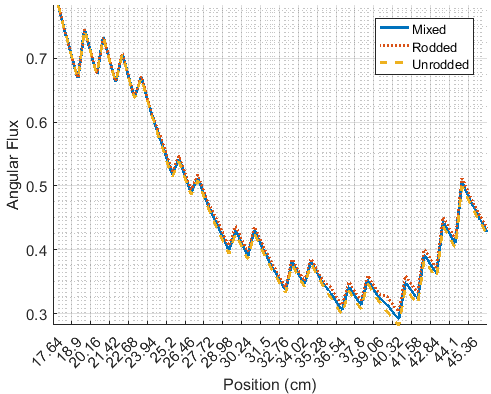
\includegraphics[width=\textwidth]{1dmoc-50mix-angflux1.png}
        \end{figure}
    \end{column}
    \begin{column}{0.4\textwidth}
        \begin{figure}[H]
            \centering
            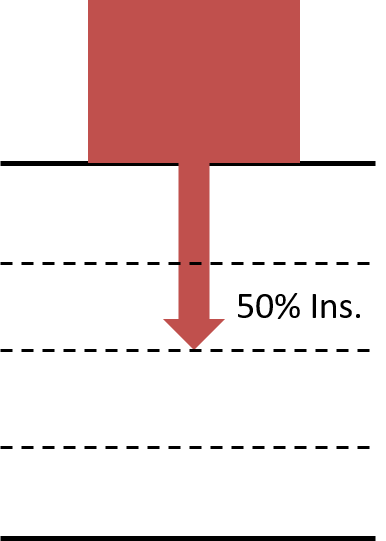
\includegraphics[width=0.75\textwidth]{rodInsertion-50percent.png}
        \end{figure}
    \end{column}
\end{columns}

\end{frame}

%%%%%%%%%%%%%%%%%%%%%%%%%%%%%%%%%%%%%%%%%%%%%%%%%%%%%%%%%%%%%%%%%%%%%%%%%%%%%%%%%

\begin{frame}[t]{Fixed Fission Source}

\begin{columns}
    \begin{column}{0.6\textwidth}
        \begin{itemize}
            \item Angular Flux, Group 1, 75\% rodded
        \end{itemize}
        \begin{figure}[H]
            \centering
            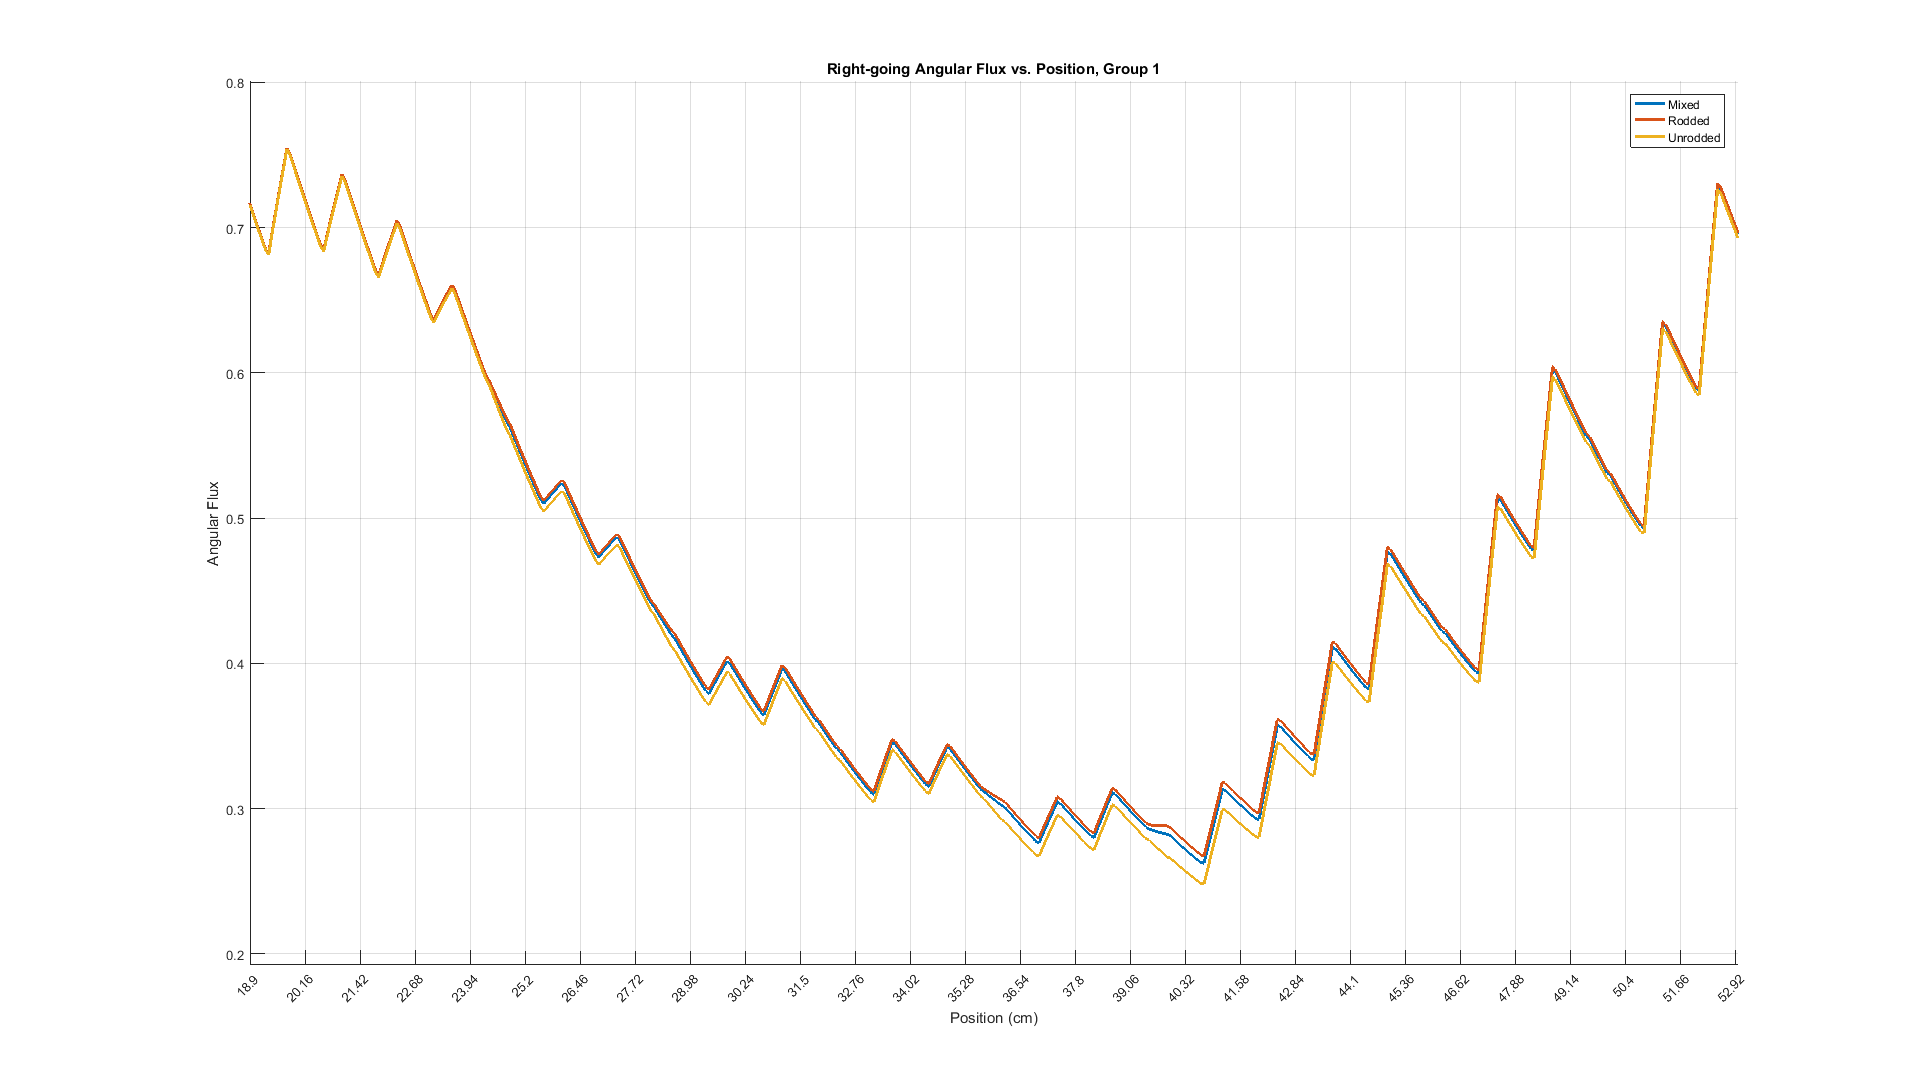
\includegraphics[width=\textwidth]{1dmoc-75mix-angflux1.png}
        \end{figure}
    \end{column}
    \begin{column}{0.4\textwidth}
        \begin{figure}[H]
            \centering
            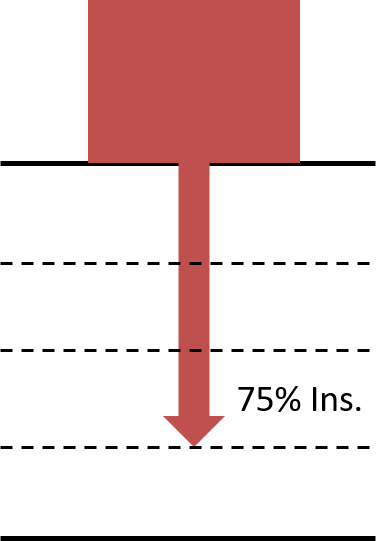
\includegraphics[width=0.75\textwidth]{rodInsertion-75percent.png}
        \end{figure}
    \end{column}
\end{columns}

\end{frame}

%%%%%%%%%%%%%%%%%%%%%%%%%%%%%%%%%%%%%%%%%%%%%%%%%%%%%%%%%%%%%%%%%%%%%%%%%%%%%%%%%

\begin{frame}[t]{1D MOC Summary}
    
    \begin{itemize}
        \item Fixed total source
        \begin{itemize}
            \item Differences between rodded and unrodded thermal flux are only significant in partially rodded cell
            \item Fast fluxes differences are small, but last much longer
        \end{itemize}
        \item Fixed fission source
        \begin{itemize}
            \item Scattering source in neighboring pins changes significantly depending on partially rodded cell
            \item If angular flux exiting partially rodded cells is treated, neighboring pin cells will not be affected by cusping
            \item Need to capture difference between rodded and unrodded angular flux
        \end{itemize}
    \end{itemize}
    
\end{frame}

%%%%%%%%%%%%%%%%%%%%%%%%%%%%%%%%%%%%%%%%%%%%%%%%%%%%%%%%%%%%%%%%%%%%%%%%%%%%%%%%%

\begin{frame}[t]{Sub-Ray MOC Method}
    
    \begin{itemize}
        \item Perform standard 2D MOC calculations in pin cells with no cusping effects
        \item For partially rodded pin cells, use multiple ``sub-rays'' to capture partially rodded effects
        \begin{itemize}
            \item Use sub-planes to determine sources for rodded and unrodded regions
            \item Determine angular flux with rodded cross-section and source; repeat with unrodded values
            \item Average rodded and unrodded angular flux for each ray segment
        \end{itemize}
        \item Angular flux exiting pin cell will prevent cusping effects in neighboring cells
        \item Currents used for sub-plane CMFD $\hat{D}$ can be calculated using explicit rodded and unrodded angular fluxes
        \item Sub-rays could be used for other reactor components such as spacer grids, burnable poison inserts, etc.
    \end{itemize}
    
\end{frame}

%%%%%%%%%%%%%%%%%%%%%%%%%%%%%%%%%%%%%%%%%%%%%%%%%%%%%%%%%%%%%%%%%%%%%%%%%%%%%%%%%

\begin{frame}[t]{Sub-Ray MOC Method}

\begin{figure}
    \centering
    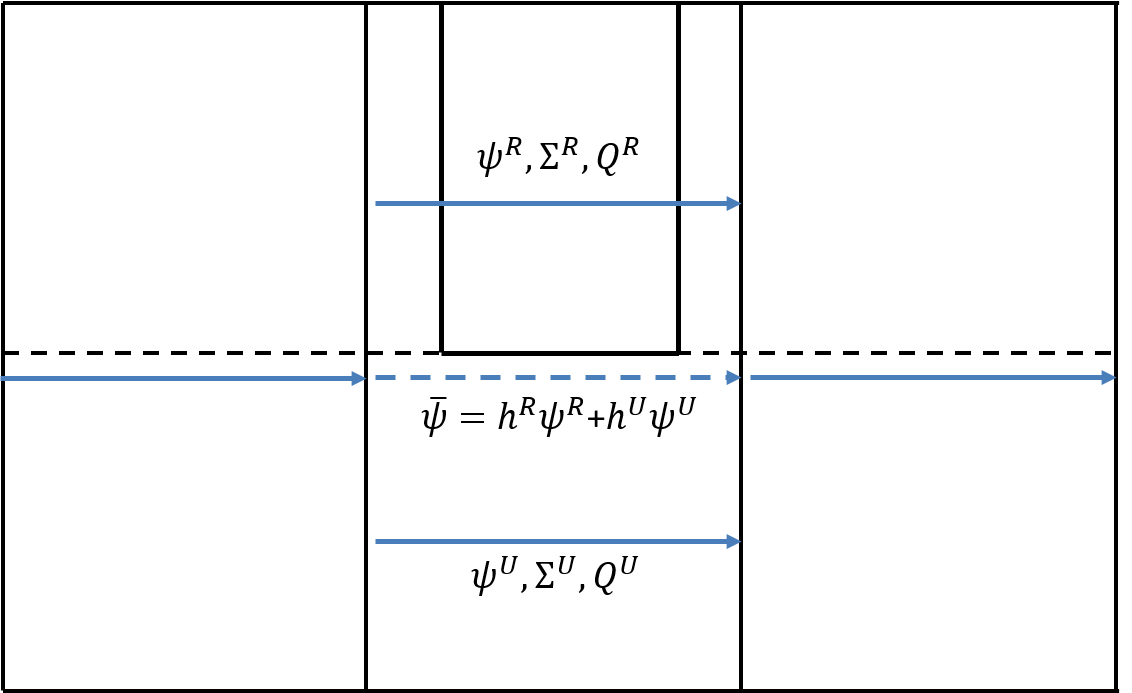
\includegraphics[width=0.8\textwidth]{sub-ray_illustration.png}
\end{figure}

\end{frame}